% ============================================================
% Figure 1: System Overview Schematic — POMDP Sea Lice Management
% Compile: pdflatex system_overview_schematic.tex
% ============================================================
\documentclass[border=8pt]{standalone}
\usepackage[T1]{fontenc}
\usepackage{tikz}
\usepackage{amsmath,amssymb}
\usepackage{booktabs}
\usepackage{array}

\usetikzlibrary{
  arrows.meta,
  shapes.geometric,
  positioning,
  fit,
  backgrounds,
  calc,
  decorations.pathreplacing
}

% ---- Action colors (match PLOS_ACTION_STYLE_ORDERED) ----
\definecolor{actNone}{HTML}{4169B0}   % blue!70!black
\definecolor{actMech}{HTML}{2B8C8C}   % teal!75!black
\definecolor{actChem}{HTML}{D98C0A}   % orange!85!black
\definecolor{actTherm}{HTML}{CC3333}  % red!80!black

% ---- Node fill colors (low-saturation pastels) ----
\definecolor{fillState}{HTML}{D6E6F0}
\definecolor{fillObs}{HTML}{F5E6C8}
\definecolor{fillBelief}{HTML}{D0E8D8}
\definecolor{fillPolicy}{HTML}{DDD4EA}
\definecolor{fillAction}{HTML}{E8E8E8}
\definecolor{fillDyn}{HTML}{CCE5E5}

% ---- Border colors ----
\definecolor{bordState}{HTML}{3A7CA5}
\definecolor{bordObs}{HTML}{C49530}
\definecolor{bordBelief}{HTML}{4A9B6E}
\definecolor{bordPolicy}{HTML}{7B5EA7}
\definecolor{bordAction}{HTML}{888888}
\definecolor{bordDyn}{HTML}{2B8C8C}
\definecolor{pipeGray}{HTML}{6B7B8D}

% ---- Styles ----
\tikzset{
  mainbox/.style={
    rectangle, rounded corners=4pt,
    minimum width=2.8cm, minimum height=1.8cm,
    text centered, text width=2.7cm,
    font=\footnotesize, align=center,
    line width=0.6pt
  },
  statebox/.style={mainbox, fill=fillState, draw=bordState},
  obsbox/.style={mainbox, fill=fillObs, draw=bordObs},
  beliefbox/.style={mainbox, fill=fillBelief, draw=bordBelief},
  policybox/.style={mainbox, fill=fillPolicy, draw=bordPolicy},
  actionbox/.style={mainbox, fill=fillAction, draw=bordAction},
  dynbox/.style={mainbox, fill=fillDyn, draw=bordDyn},
  pipebox/.style={
    rectangle, rounded corners=3pt,
    minimum width=7.0cm, minimum height=1.5cm,
    text centered, text width=6.6cm,
    font=\footnotesize, align=center,
    draw=pipeGray!60, line width=0.5pt, fill=pipeGray!8
  },
  annotbox/.style={
    rectangle, rounded corners=3pt,
    font=\footnotesize, align=left,
    draw=black!35, line width=0.4pt, fill=white,
    inner sep=7pt
  },
  loopedge/.style={-{Stealth[length=5pt]}, line width=0.7pt, color=black!70},
  pipeedge/.style={-{Stealth[length=5pt]}, line width=0.8pt, color=pipeGray!80, densely dashed},
  steplabel/.style={
    circle, draw=black!50, fill=white, inner sep=0pt,
    minimum size=13pt, font=\scriptsize\bfseries, text=black!70
  }
}

\begin{document}
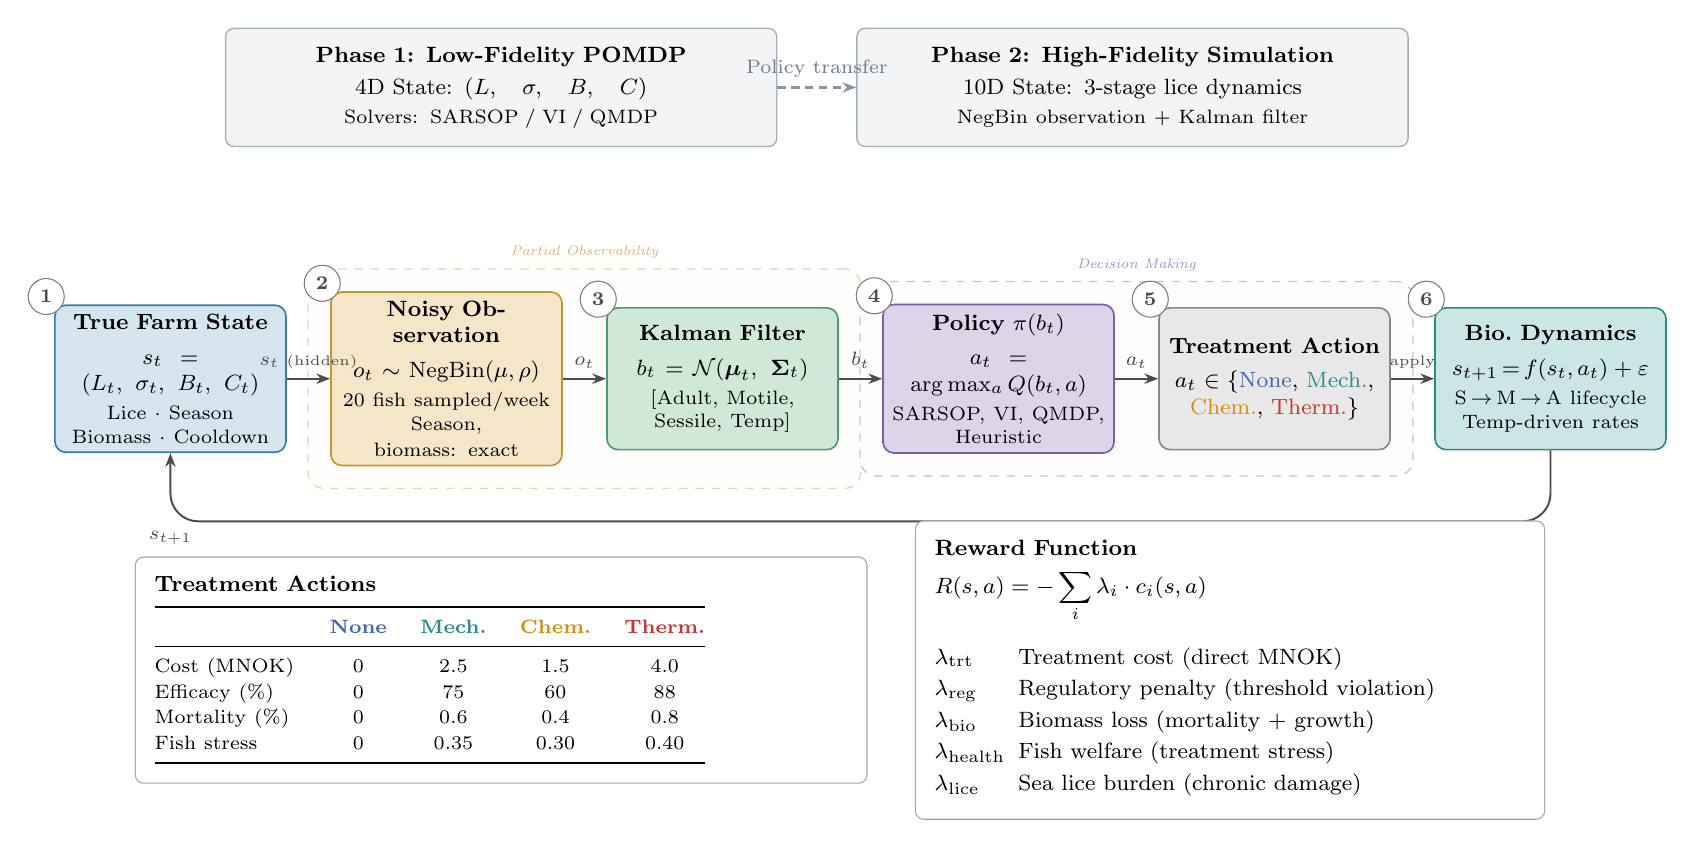
\begin{tikzpicture}[node distance=0.45cm and 0.45cm]

% ================================================================
%  ZONE A: Solve-then-Simulate Pipeline (top)
% ================================================================
\node[pipebox] (lofi) at (4.2, 9.2) {%
  \textbf{Phase 1: Low-Fidelity POMDP}\\[2pt]
  4D State: $(L,\;\sigma,\;B,\;C)$\\[1pt]
  {\scriptsize Solvers: SARSOP\;/\;VI\;/\;QMDP}
};

\node[pipebox, right=1.0cm of lofi] (hifi) {%
  \textbf{Phase 2: High-Fidelity Simulation}\\[2pt]
  10D State: 3-stage lice dynamics\\[1pt]
  {\scriptsize NegBin observation + Kalman filter}
};

\draw[pipeedge] (lofi) -- node[above, font=\scriptsize, text=pipeGray] {Policy transfer} (hifi);

% ================================================================
%  ZONE B: Central POMDP Decision Loop (middle)
% ================================================================

% --- Node 1: True Farm State ---
\node[statebox] (state) at (0, 5.5) {%
  \textbf{True Farm State}\\[3pt]
  $s_t = (L_t,\;\sigma_t,\;B_t,\;C_t)$\\[1pt]
  {\scriptsize Lice $\cdot$ Season}\\[-1pt]
  {\scriptsize Biomass $\cdot$ Cooldown}
};

% --- Node 2: Noisy Observation ---
\node[obsbox, right=0.55cm of state] (obs) {%
  \textbf{Noisy Observation}\\[3pt]
  $o_t \sim \mathrm{NegBin}(\mu,\rho)$\\[1pt]
  {\scriptsize 20 fish sampled/week}\\[-1pt]
  {\scriptsize Season, biomass: exact}
};

% --- Node 3: Kalman Filter Belief ---
\node[beliefbox, right=0.55cm of obs] (belief) {%
  \textbf{Kalman Filter}\\[3pt]
  $b_t = \mathcal{N}(\boldsymbol{\mu}_t,\;\boldsymbol{\Sigma}_t)$\\[1pt]
  {\scriptsize [Adult, Motile,}\\[-1pt]
  {\scriptsize Sessile, Temp]}
};

% --- Node 4: Policy ---
\node[policybox, right=0.55cm of belief] (policy) {%
  \textbf{Policy $\pi(b_t)$}\\[3pt]
  $a_t = \arg\max_a Q(b_t,a)$\\[1pt]
  {\scriptsize SARSOP, VI, QMDP,}\\[-1pt]
  {\scriptsize Heuristic}
};

% --- Node 5: Treatment Action ---
\node[actionbox, right=0.55cm of policy] (action) {%
  \textbf{Treatment Action}\\[3pt]
  $a_t \in \{$%
  \textcolor{actNone}{None},
  \textcolor{actMech}{Mech.},\\
  \textcolor{actChem}{Chem.},
  \textcolor{actTherm}{Therm.}$\}$
};

% --- Node 6: Biological Dynamics ---
\node[dynbox, right=0.55cm of action] (dyn) {%
  \textbf{Bio.\ Dynamics}\\[3pt]
  $s_{t+1}\!=\!f(s_t,a_t)+\varepsilon$\\[1pt]
  {\scriptsize S\,$\to$\,M\,$\to$\,A lifecycle}\\[-1pt]
  {\scriptsize Temp-driven rates}
};

% --- Step number labels (positioned outside top-left corner) ---
\node[steplabel] at ($(state.north west)+(-0.1, 0.1)$)  {1};
\node[steplabel] at ($(obs.north west)+(-0.1, 0.1)$)    {2};
\node[steplabel] at ($(belief.north west)+(-0.1, 0.1)$) {3};
\node[steplabel] at ($(policy.north west)+(-0.1, 0.1)$) {4};
\node[steplabel] at ($(action.north west)+(-0.1, 0.1)$) {5};
\node[steplabel] at ($(dyn.north west)+(-0.1, 0.1)$)    {6};

% --- Forward arrows ---
\draw[loopedge] (state)  -- node[above, font=\scriptsize] {$s_t$ \tiny(hidden)} (obs);
\draw[loopedge] (obs)    -- node[above, font=\scriptsize] {$o_t$} (belief);
\draw[loopedge] (belief) -- node[above, font=\scriptsize] {$b_t$} (policy);
\draw[loopedge] (policy) -- node[above, font=\scriptsize] {$a_t$} (action);
\draw[loopedge] (action) -- node[above, font=\scriptsize] {\tiny apply} (dyn);

% --- Feedback arrow (curves below) ---
\draw[loopedge, rounded corners=10pt]
  (dyn.south) -- ++(0,-0.9) -| (state.south)
  node[pos=0.5, below, font=\scriptsize] {$s_{t+1}$};

% ================================================================
%  ZONE C: Annotation Panels (bottom)
% ================================================================

% --- Left panel: Treatment Actions ---
\node[annotbox, text width=8.8cm] (trtpanel) at (4.2, 1.8) {%
  \textbf{Treatment Actions}\\[4pt]
  \renewcommand{\arraystretch}{1.15}%
  {\scriptsize
  \begin{tabular}{@{}>{\raggedright}p{1.8cm} c c c c@{}}
    \toprule
    & \textcolor{actNone}{\textbf{None}}
    & \textcolor{actMech}{\textbf{Mech.}}
    & \textcolor{actChem}{\textbf{Chem.}}
    & \textcolor{actTherm}{\textbf{Therm.}} \\
    \midrule
    Cost (MNOK)    & 0   & 2.5  & 1.5  & 4.0  \\
    Efficacy (\%)  & 0   & 75   & 60   & 88   \\
    Mortality (\%) & 0   & 0.6  & 0.4  & 0.8  \\
    Fish stress    & 0   & 0.35 & 0.30 & 0.40 \\
    \bottomrule
  \end{tabular}}
};

% --- Right panel: Reward Components ---
\node[annotbox, text width=7.5cm, right=0.6cm of trtpanel] (rwdpanel) {%
  \textbf{Reward Function}\\[4pt]
  $R(s,a) = -\displaystyle\sum_{i}\lambda_i \cdot c_i(s,a)$\\[6pt]
  \renewcommand{\arraystretch}{1.2}%
  \begin{tabular}{@{}l@{\;\;}l@{}}
    $\lambda_{\text{trt}}$    & Treatment cost (direct MNOK) \\
    $\lambda_{\text{reg}}$    & Regulatory penalty (threshold violation) \\
    $\lambda_{\text{bio}}$    & Biomass loss (mortality + growth) \\
    $\lambda_{\text{health}}$ & Fish welfare (treatment stress) \\
    $\lambda_{\text{lice}}$   & Sea lice burden (chronic damage) \\
  \end{tabular}
};

% ================================================================
%  Dashed grouping boxes (optional visual aid)
% ================================================================
\begin{pgfonlayer}{background}
  % Partial observability group
  \node[rounded corners=6pt, draw=bordObs!40, dashed, line width=0.5pt,
        fill=fillObs!5, inner sep=8pt,
        fit=(obs)(belief),
        label={[font=\tiny\itshape, text=bordObs!70]above:Partial Observability}] {};
  % Decision group
  \node[rounded corners=6pt, draw=bordPolicy!40, dashed, line width=0.5pt,
        fill=fillPolicy!5, inner sep=8pt,
        fit=(policy)(action),
        label={[font=\tiny\itshape, text=bordPolicy!70]above:Decision Making}] {};
\end{pgfonlayer}

\end{tikzpicture}
\end{document}
